\section{Kravspecifikationer}
Dette afsnit vil indeholde en beskrivelse af systemet og kravspecifikationer til systemets indeholde. 

\subsection{Systemets funktion}
Systemet har til formål at hjælpe apopleksipatienter med balanceproblemer ved at give patienten besked, når kroppen ikke er i balance. Dette skal afværge faldulykker, som apopleksipatienter har stor risiko for at opleve.

Overordnet skal systemet kunne bestemme patientens kropshældning og give besked hvis patienten kommer ud af balance vha. signaler. Dette vil forgå således, at når patienten begynder at hælde til en side, vil en diode lyse og der vil lyde en alarm indtil patienten har rettet kroppen på plads. 

\subsection{System krav}
\begin{itemize}
\item Systemet skal anvendes visuel og auditiv feedback 
\item Systemet skal være non-invasiv - dvs. systemet må ikke påføre patienten smerte eller varig skade
\item Systemet skal være brugervenlig
\item Systemet skal forsynes med spænding fra et batteri
\end{itemize}

\subsection{Blokdiagram}
Her vil der komme en beskrivelse af de enkelte blokke, som systemet skal indeholde, hvilket fremgår af \figref{krav_blok}.

\begin{figure}[H]
	\centering
	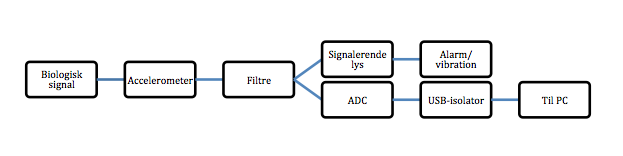
\includegraphics[scale=0.8]{figures/bProblemanalyse/Kravspecifikationer - blokdiagram.png}
	\caption{Figuren viser de blokke/elementer som systemet skal indeholde}
	\label{krav_blok}
\end{figure}

\subsubsection{Accelerometer}
Accelerometeret skal detektere patientens kropshældning.

\subsubsection{Filter}
Når der anvendes et filter, skal det dæmpe uønskede frekvenser. Dvs. frekvenser der lavere eller højere ift. det signal fra accelerometeret, som man vil analysere på. Der skal udføres et pilotforsøg for at finde frem til det korrekte filter og valg af knækfrekvens. 

\subsubsection{Signalerende lys}
Når patienten er ude af balance skal en rød diode lyse, som signalering ift. patientens hældning. Der skal vha. et pilotforsøg detekteres, hvornår dioden skal lyse. Skal der evt. være 2 dioder, hvor den ene er et "advarende" signal og nr. to er "fare". 

\subsubsection{Alarm/vibrationen}
Alarmen/vibrationen skal anvendes i perioden, hvor patienten er ude af balance og stoppe igen, når der igen er oprettet balance. 
(eller fungere som en alarm til dioderne - så når en diode lyser, skal alarmen gå)

\subsubsection{ADC}
Der anvendes en ADC i systemet, for at konvertere det analoge signal til digitalt. Det næste skridt er konverteringen til PC og det er derfor essentielt at have en ADC, der konverterer analogt signal til binære tal, som digitale systemet anvender. 
{Her skal vi have valgt en samplingsfrekvens)

\subsubsection{USB-isolater}
USB-isolatoren sikre patientens sikkerhed. Her skal input- og outputspænding være ens.  

\subsubsection{Til PC}
Fremvisning af graf, så patienten og plejepersonale kan følge rehabiliteringens udvikling. 

% Inspiration især fra: Brug af Biofeedback til Rehabilitering af Apopleksipatienter 